%!TEX root = ../main.tex

\chapter{UMAP} 

\label{UMAP} 

%----------------------------------------------------------------------------------------

% N O T I Z E N
% Wirkung des Funktors beschreiben \cite{Posada}
% Bisher: Daten -> metr. R�ume -> fuzzy simplicial sets
% Ziel:   Daten -> metr. R�ume -> VR complex

% T E X T B A U S T E I N E
% 

%----------------------------------------------------------------------------------------
%----------------------------------------------------------------------------------------

% \section{Einleitung}
In diesem Kapitel werden wir die aus \ref{Grundlagen} erlangten Grundlagen verwenden um 
eine geeignete topologische Repr�sentation unserer Daten $X=\seqx$ zu erlangen. Eine �hnliche 
Repr�sentation werden wir von einem $d$-dimensionalen Raum $(d \ll D)$ betrachten, um dann mit einem geeigneten 
Begriff des Abstandes der beiden Repr�sentationen die niedrigdimensionale Repr�sentation der 
hochdimensionalen anzupassen. Dies wird uns zum UMAP Verfahren f�hren. 
% TODO: Erg�nzungen hier erw�hnen oder in \ref{Implementierung}?

%----------------------------------------------------------------------------------------

\section{Topologische Repr�sentation}
	Blabla bla

%-----------------------------------

	\subsection*{Fluch der Dimensionen}
	% Zitiere Bengio 2007
	Ein kritischer Punkt beim analysieren hochdimensionaler Daten ist der sogenannte Fluch der Dimensionen.
	Was das bedeutet und wie das UMAP Verfahren macht um diesen zu vermeiden werde ich im Folgenden kurz erkl�ren.
	Unter dem Fluch der Dimensionen versteht man.
	% D�nn besetzt ist schlecht, da keine Stetigkeit mehr, besonders bei lokalen eigenschaften wichtig 


	Abbildung \ref{fig:Curse} kann man zwei interessante Aussagen �ber den Fluch der Dimensionen entnehmen. 
	% TODO: enumerate einf�gen?
	\begin{enumerate}
	\item Die paarweisen euklidischen Distanzen steigen mit zunehmender Gr��e der Dimensionen. 
	\item Die paarweisen Distanzen sind ungef�hr normalverteilt, wobei die Varianz der Normalverteilung f�r h�here 
		Dimensionen abnimmt. Dadurch sind die Distanzen eines Punktes zu seinen ersten, zweiten, \dots k-ten Nachbarn 
		im hochdimensionalen Raum ann�hernd gleich. 
	\end{enumerate}

	\begin{figure}
		%\centering
		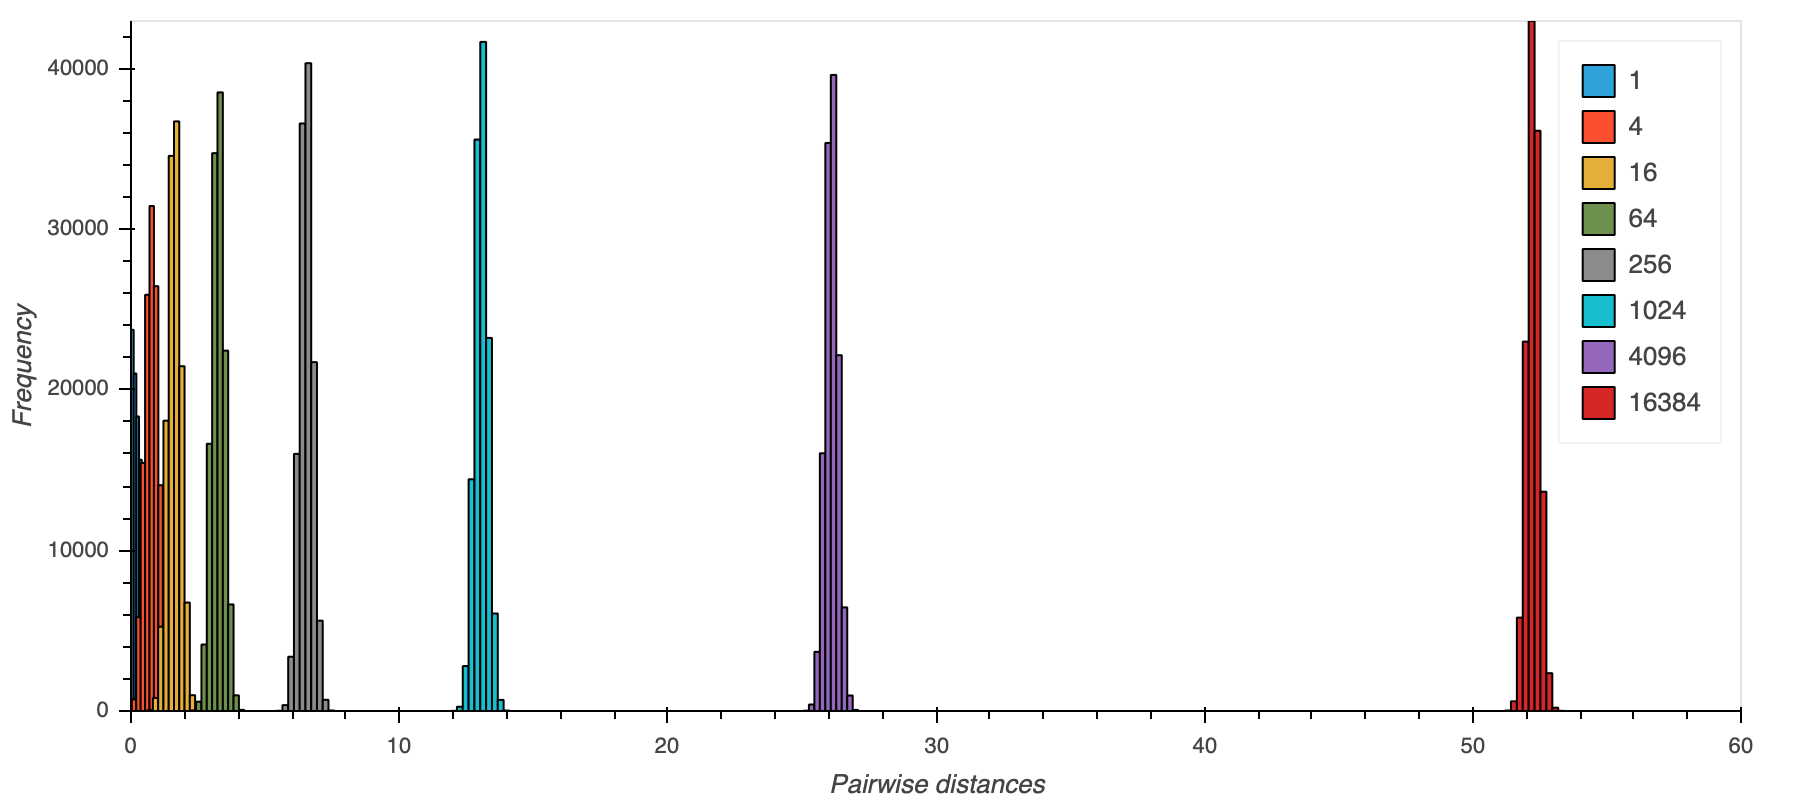
\includegraphics[width=400px, height=178px]{Figures/pairwise_dist}
		%\decoRule
		\caption[Durchsch. Distanz]{Paarweise Distanzen von $N=500$ zuf�llig gleichverteilten Punkten im $R^D$.}
		\label{fig:Curse}
	\end{figure}

	Um dieses Ph�nomen zu vermeiden nutzt das UMAP Verfahren eine Normalisierung der Distanzen mit dem ersten 
	Nachbarn. So werden die relativen Distanzen zwischen den k-n�chsten-Nachbarn gr��er, siehe %TODO: f�ge Grafik ein


	Um die niedrigdimensionale Repr�sentation der hochdimensionalen anzupassen wird f�r das UMAP Verfahren die 
	Kreuzentropie zwischen zwei unsicheren (simplizialen) Mengen vorgeschlagen. 
	
	\begin{equation}
		C((A,\mu), (A, \nu)) \coloneqq \sum_{a \in A} \left(\mu(a)\log\left(\frac{\mu(a)}{\nu(a)}\right) +  \left(1-\mu(a)\right)\log\left(\frac{1-\mu(a)}{1-\nu(a)}\right)  \right)
		\label{eq:crossentropy}
	\end{equation}
	
	In Abschnitt \ref{seq:numerische_formulierung} werden wir die Kreuzentropie genauer betrachten.

%----------------------------------------------------------------------------------------

\section{Erg�nzungen}

% Wenn VR Komplex ausreichend, betrachte nur 1-Skelet und berechne Homologie darauf.
% Siehe Oudot s.48, funktioniert noch nicht f�r Filtrationen. 

